\documentclass[10pt,a4paper]{article}
\usepackage[latin1]{inputenc}
\usepackage{amsmath}
\usepackage{amsfonts}
\usepackage{amssymb}
\usepackage{graphicx}
\usepackage[margin=1in]{geometry}
\usepackage{siunitx}

\usepackage{float}
\usepackage{subcaption}

\title{EELE 582 Optical Design \\ Homework 4 \\Designing a Landscape Lens }
\author{Roy Smart}
\begin{document}
	
\maketitle	

\section{Determining Initial Configuration} \label{init}

	For our initial lens system, we will start with an equiconvex lens. The curvature of this lens, $R=R1=-R2$ is given by the following
	\begin{align*}
		R &=2 (n - 1) f_E \\
		&= 2 (1.5168 - 1) (\SI{100}{\milli\meter}) \\
		&= \SI{103.36}{\milli\meter}
	\end{align*}
	In our Zemax model, we will start with an equiconvex lens, with a radius of curvature of $\pm$103.36mm, and a thickness of 4mm. The stop will be placed approximately $f/2=\SI{50}{\milli \meter}$ from the back surface of the lens and the clear semi-diameter will be scaled such that the $f/\# = 15$.

\section{Zemax Configuration}
	\subsection{Aperature} \label{aper}
	
		To float the aperture according to  $f/\#$ we navigate to the Aperture section of the System Explorer, select the Aperature Type to be Image Space $f/\#$, and set the Aperature Value to be 15. All surfaces in the optical system will now adjust their size according to the $f/\#$.

	\subsection{Fields and Wavelengths}
	
		We will need to add additional fields to explore the off-axis performance of this system. We can do this by navigating to the Fields section of the System Explorer. We will keep Field 1 at its default values. We will add two new fields, Field 2 and Field 3. The Y-values of these fields will be 10.5 and 15.0 respectively. This configuration will provide raytrace information from field angles of 0, 10.5, and 15 degrees.
		
		We are asked to use a different wavelength than Zemax's default wavelength. To edit this parameter we navigate to the Wavelengths Section of the System Explorer. Here we may set the value of Wavelength 1 to be \SI{0.587}{\micro\meter}.
	
	\subsection{Initial Surfaces}
	
		Based off of the description in Section \ref{init} we will enter our optical system into Zemax with the values given in Table \ref{init_v}. The Clear Diameter for all surfaces is set by the Aperature Type in Section \ref{aper}.	
		
		Surface 1 is a dummy surface, used to observe the incoming rays. In the Surface 1 Properties we check `Do Not Draw This Surface', which makes the surface transparent in the Layout.
		
		Surface 2 is the front of the lens. It is initially set to the curvature determined in Section \ref{init}, and the thickness is given in the problem statement as \SI{4}{\milli \meter}. The curvature of this surface will be found by the optimizer, so we set it as a variable.
		
		Surface 3 is the back of the lens. Similar to the front surface it is set to negative the curvature determined in Section \ref{init}. An initial thickness of the lens was chosen to be $f/2=\SI{50}{\milli \meter}$. The curvature and thickness of this lens are to be found by the optimizer, so both are set as variables.
		
		Surface 4 is the stop. Its thickness will be found by solving for where the marginal ray height is zero, which will place the image plane at the paraxial focus.
		
		Surface 5 is a second dummy surface. Its purpose is to allow the optimizer to add defocus, providing a compromise between focusing on-axis and off-axis. Therefore the thickness is initially 0.0, but set as a variable. Under the Surface 5 Properties we will check `Do Not Draw This Surface' and `Skip Rays To This Surface', which will prevent rays cluttering the image plane in the Layout.
	
		\begin{table}[H]
			\centering
			\begin{tabular}{r| r r r r r r r }

				Surf &      	Type     &   	Radius&     &   	Thickness&      &     	Glass     & 	  Clear Diam \\ 				\hline
				OBJ&	 STANDARD	 &      Infinity&	&       Infinity&	    &&                 	             0\\
				1	& STANDARD	   &    Infinity&	  &           30&	 U       &&             	      79.62144\\ 
				2	& STANDARD	   &     103.365&	V  &            4&	 U       &          BK7&	      61.07216\\ 
				3&	 STANDARD	   &    -103.365&	V  &           50&	 V       &&             	      64.30968\\ 
				STO	& STANDARD	   &    Infinity&	  &     49.33663&	M        &&             	      26.83858 \\ 
				5&	 STANDARD	   &    Infinity&	  &            0& V	        &&             	      108.4105\\ 
				IMA	& STANDARD	    &   Infinity&	   &&&     &       	                     	      108.4105 \\ 
			\end{tabular}
			\caption{Values for the initial lens configuration based off of paraxial calculations for an equiconvex lens.}
			\label{init_v}
		\end{table}
	
	\subsection{Merit Function} \label{mf}
	
		Start by using the optimization wizard to minimize the RMS spot size of the three field angles. Do this by setting the Type to RMS and the Reference to Centroid.
		
		Additionally, we will optimize the focal length to \SI{10}{\milli \meter} by using the \texttt{EFFL} operand, setting the value to 100.0 and the weight to 1.0.
		
		Furthermore, we will constrain the thickness of Surface 3 (the back fo the lens) to be between 0 and the focal length. This is done using the \texttt{MXCA} and \texttt{MNCA} operands, setting their weights to 1.0 and their values to 100.0 and 0.0 respectively.
	
	\subsection{Optimized Surfaces}
	
		After we run the optimizer using the Merit Function described in Section \ref{mf}, the resulting lens prescription is given by Table \ref{opti_v}. We can see that the optimizer has changed our equiconvex lens into a meniscus lens. Also, the stop has moved much closer to the lens, approximately \SI{10}{\milli \meter} from the back surface of the lens. Finally, we can see that the second dummy surface, Surface 5 has moved about \SI{2}{\milli \meter} closer to the lens. 
	
		\begin{table}[H]
			\centering
			\begin{tabular}{r| r r r r r r r }
				Surf&       	Type&        	Radius&&        	Thickness&&           	Glass&      	  Clear Diam \\ \hline
				OBJ&	 STANDARD&	       Infinity&&	       Infinity&&&                     	             0 \\
				1&	 STANDARD&	       Infinity&&	             30	  &U&&                   	      31.98845 \\
				2&	 STANDARD&	       18.40098&V&	              4	  &U &              BK7&	      15.04932 \\
				3&	 STANDARD&	       26.45827&V&	       10.89544	 &V& &                   	      12.95634 \\
				STO&	 STANDARD&	       Infinity	&&       81.69782&M&	&                     	      5.540159 \\
				5&	 STANDARD	&       Infinity&&	      -1.885163	 &V& &                   	      54.50731 \\
				IMA&	 STANDARD&	       Infinity	&&&   &            	  &                   	      53.12173 \\
			\end{tabular}
			\caption{Values for the lens configuration after running the optimizer.}
			\label{opti_v}
		\end{table}
		
		\pagebreak
	
\section{Performance}

	\subsection{Initial Configuration}
	
		In the initial lens configuration we can see that the on-axis (Field) RMS spot size is small compared to the Airy radius, however the off-axis spot size is immense compared to the Airy radius. This is immediately apparent from the layout in Figure \ref{layout_init}, but is also see in Figure \ref{spot_init}. It is also obvious from the layout that the stop is too far away to restrict the rays enough to form a good focus for all three fields.
	
		\begin{figure}[H]
			\centering
			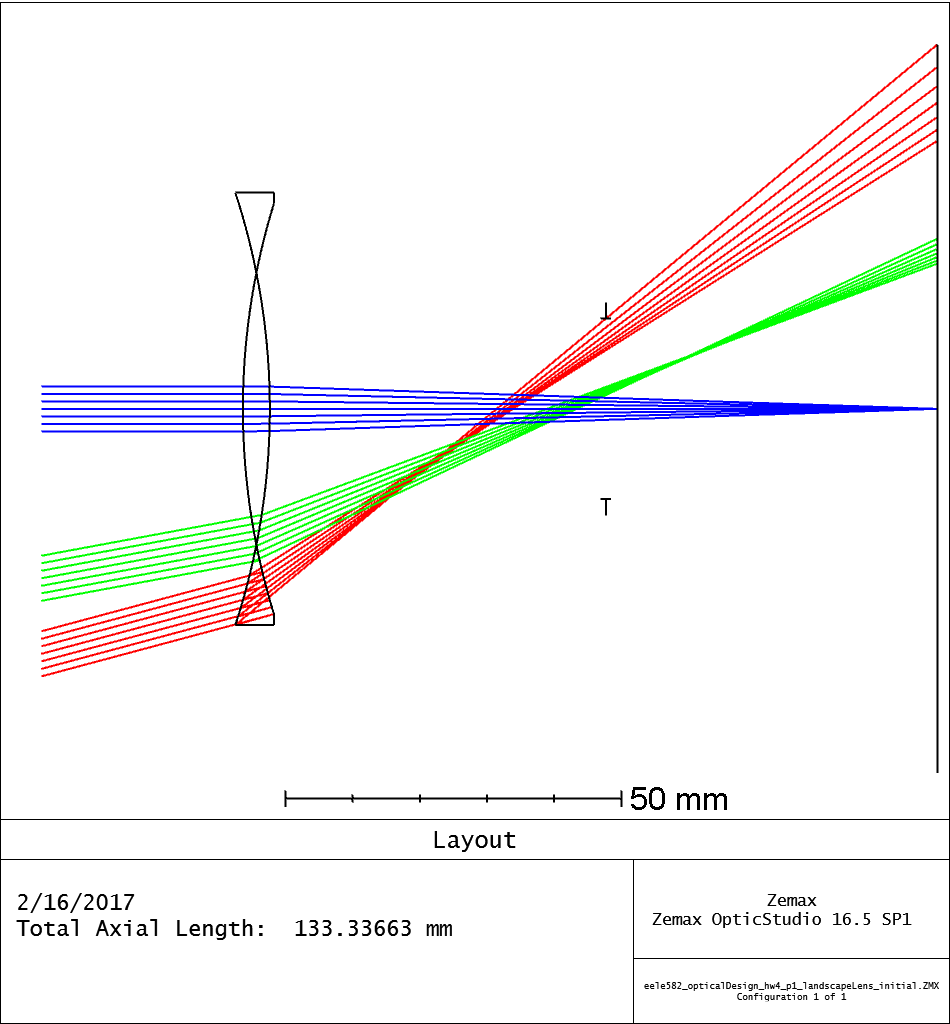
\includegraphics[width=0.5\textwidth]{../zemax/1_initial/layout}
			\caption{Layout of the initial landscape lens configuration}
			\label{layout_init}
		\end{figure}		
		\begin{figure}[H]
			\centering
			\begin{subfigure}[t]{0.5\textwidth}
				\centering
				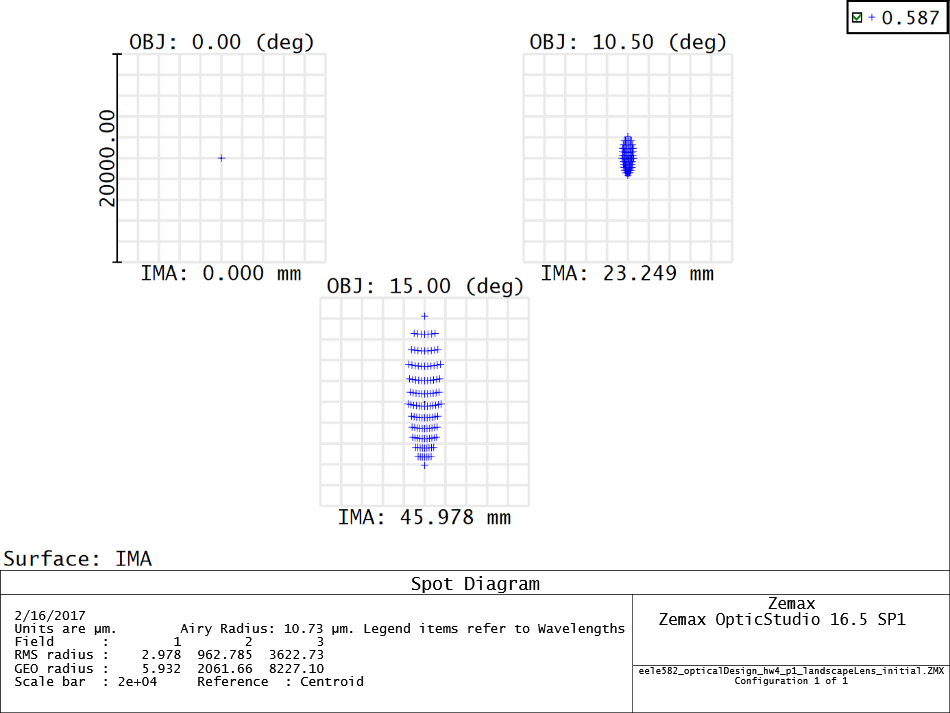
\includegraphics[width=\textwidth]{../zemax/1_initial/spot}
				\caption{Spot diagram for each field}
				\label{spot_init}
			\end{subfigure}%
			~ 
			\begin{subfigure}[t]{0.5\textwidth}
				\centering
				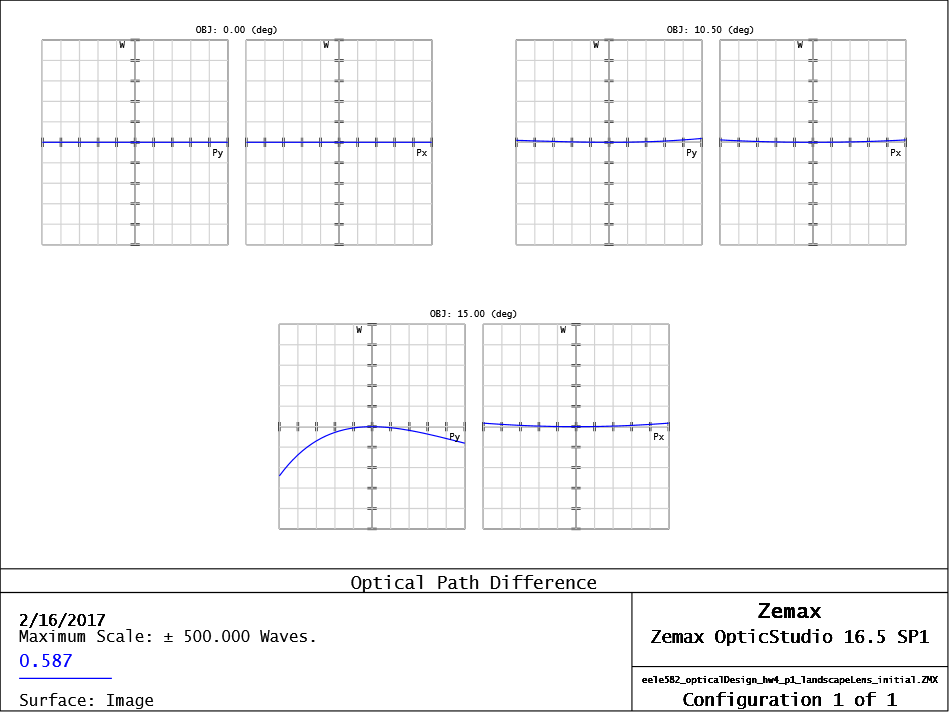
\includegraphics[width=\textwidth]{../zemax/1_initial/fan}
				\caption{Optical path difference for each field}
			\end{subfigure}
			\caption{Plots describing the performance of the initial lens configuration}
		\end{figure}
		
	\pagebreak
	\subsection{Optimized Configuration}
	
		After running the optimizer, we can see an excellent improvement in the imaging quality of our landscape lens system. From the layout in Figure \ref{layout_opto}. We can see that the rays from all three fields converge to a nice focus. 
		
		In the spot diagram in Figure \ref{spot_opto} we can take a closer look at the focus formed by each field. Field 1 has some spherical aberration as evidenced by the rings formed in its spot diagram. Field 2 is the best of the three fields in terms fo RMS spot size, and exhibits only slight astigmatism. Field 3 has the worst RMS spot size, and is plagued by astigmatism, demonstrated by the elliptic halo around the central spot.
		
		All three of our fields were within the specifications provided by Geary for RMS spot sizes at these field angles.
	
		\begin{figure}[H]
			\centering
			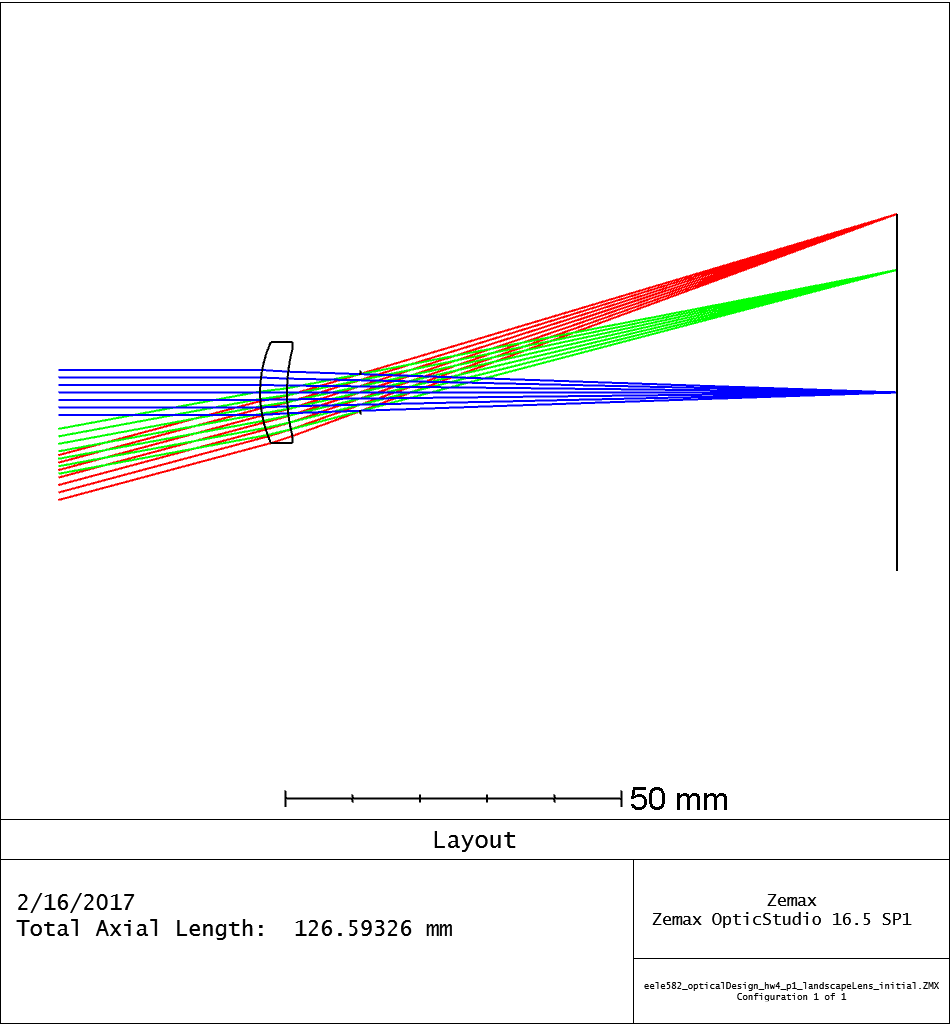
\includegraphics[width=0.5\textwidth]{../zemax/2_optimized/layout}
			\caption{Layout of the optimized landscape lens configuration}
			\label{layout_opto}
		\end{figure}		
		\begin{figure}[H]
			\centering
			\begin{subfigure}[t]{0.5\textwidth}
				\centering
				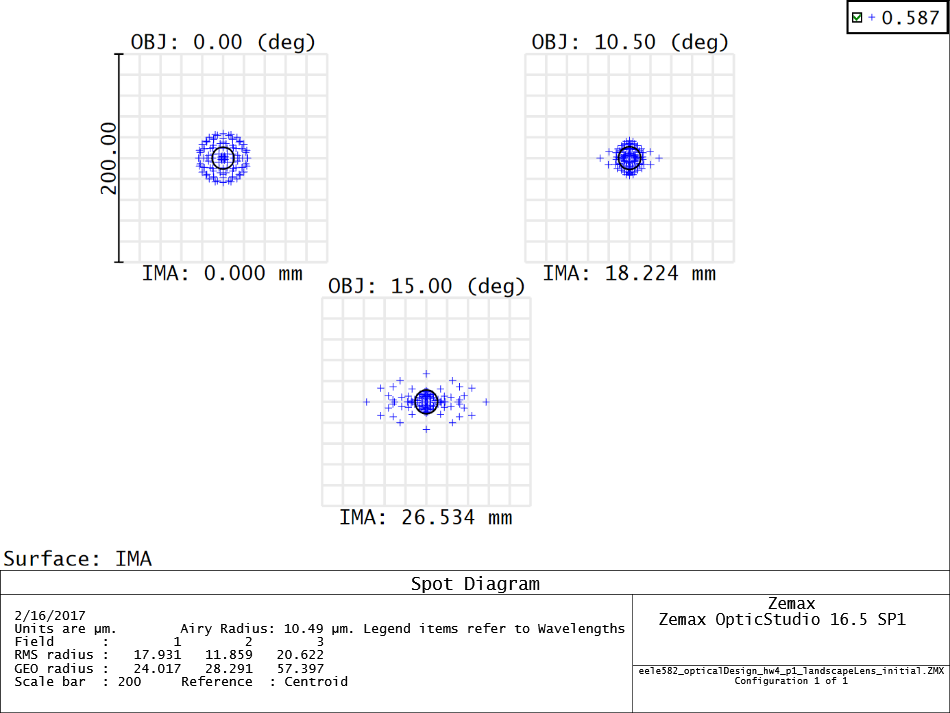
\includegraphics[width=\textwidth]{../zemax/2_optimized/spot}
				\caption{Spot diagram for each field}
				\label{spot_opto}
			\end{subfigure}%
			~ 
			\begin{subfigure}[t]{0.5\textwidth}
				\centering
				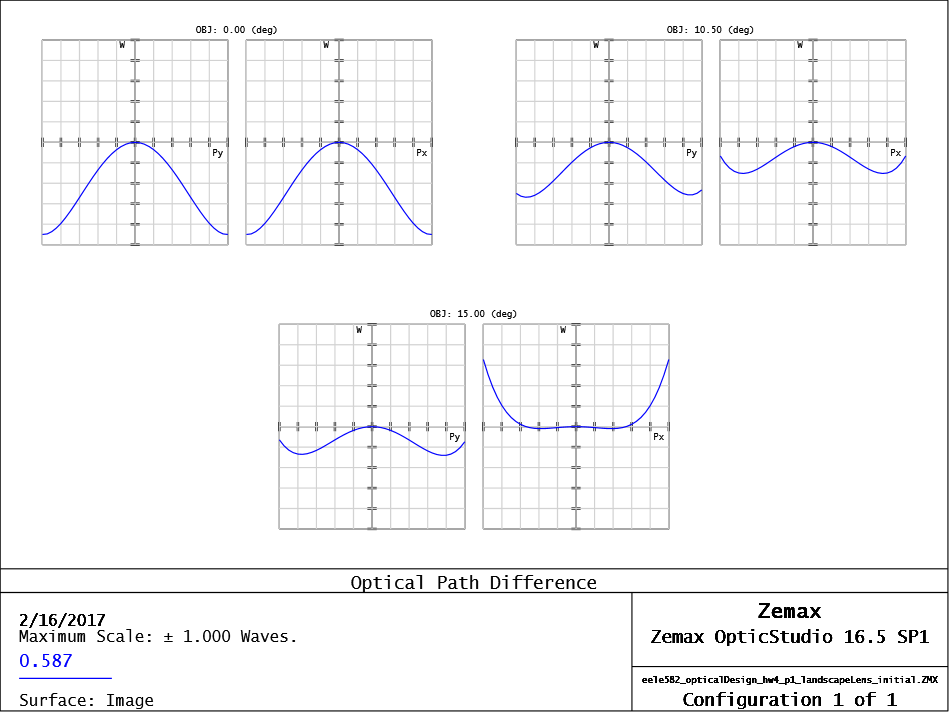
\includegraphics[width=\textwidth]{../zemax/2_optimized/fan}
				\caption{Optical path difference for each field}
			\end{subfigure}
			\caption{Plots describing the performance of the optimized lens configuration}
		\end{figure}

\pagebreak

\section{Lessons Learned}

In this project, we learned about using the Aperature Type `Image Space F/\#' to restrict light to the appropriate $f/\#$. We also learned about the solvers available for different parameters in the Lens Data Editor, such as the marginal ray height solver, used to find the paraxial image plane.

Finally, we learned about the optimizer. We tried to familiarize ourselves with some of the operands available to us, and used the optimization wizard to automate the creation of these operands. We learned how to specify variables in the Lens Data Editor.
	
\end{document}